\documentclass[../thesis.tex]{subfiles}
% Separate preamble for this subfile. This preamble is loaded last, so one can override various functions before \begin{document}

% Better comment extension for Vscode colors these comments differently
% Normal comment color
% * Important information
% ! ALERT
% ? Question
% TODO stuff to do
% // this is strikethrough


\begin{document}

Before tackling spectral sets in higher dimensions, we first emphasize the importance of \cref{eq:zero_set_equation} and generalize it to higher dimensions. 
\begin{lemma}
    Let $\Omega=I^d$. The zero-set for the function
    \begin{equation*}
        F_{\Omega} (z):= \int_\Omega e^{2 \pi i \braa{z,t}} dt  = \int_\Omega e^{2 \pi i \braa{(\lambda-\lambda'),t}} dt = \braaMed{e_{\lambda},e_{\lambda'} }_{L^2(I^d)}
    \end{equation*}
    is the following set
    \begin{equation*}
        \Zstroke_{I^d} = \braqMed{ z = \brac{z_1,\dots,z_d}\in \C^d \setminus \braqMed{0} : \exists \space j \in \braqMed{1,\dots, d} \text{ such that } z_j \in  \Z\setminus \braqMed{0}}
    \end{equation*}
\end{lemma}

\begin{example}
    The zero-set for $F_{\Omega}$ when $d=1$ is the following
    \begin{equation*}
        \Zstroke_{I} = \braqMed{ z \in \C \setminus \braqMed{0} : \exists \space z \in  \Z\setminus \braqMed{0}} = \Z 
    \end{equation*}
\end{example}

\begin{proof}
    
\end{proof}

\begin{remark}
    Given a spectral pair $(I^d,\Lambda)$ and the following set 
    \begin{equation*}
        \Lambda - \Lambda = \braqMed{\lambda-\lambda' : \lambda,\lambda' \in \Lambda}.
    \end{equation*}
    Then it follows that the spectral pair property is equivalent to the non-zero elements of $\Lambda - \Lambda$ being contained in the zero-set of $F_{\Omega}$. More specifically, if $(I^d,\Lambda)$ is a spectral pair, then
    \begin{equation*}
        \Lambda - \Lambda \subset \Z_{I^d} \cup \braq{0}. 
    \end{equation*}
\end{remark}

\begin{example}
    Observe that for $\Lambda=\Z$, the non-zero elements of $\Lambda - \Lambda$ is $\Z\setminus \braq{0}$
\end{example}


%! BEGYN HER
%* —————————————————————————————————————


In \cite{jorgensenSpectralPairsCartesian2001}, Pedersen and Jorgensen present a way of constructing spectral pairs in higher dimensions from spectral pairs in lower dimensions. 

\begin{theorem}[Construction of spectra]\label{thrm:construction_spectra}
    Let $\brac{\Omega_1,\Lambda_1}$ be a spectral pair in dimension $d_1$, and let $\Omega_2$ be a set of positive finite measure in dimension $d_2$. Suppose for each $\lambda_1 \in \Lambda_1$ that $\lambfunc$ is a discrete subset of $\R^{d_2}$ such that $\brac{\Omega_2,\lambfunc}$ is a spectral pair. If 
    \begin{equation*}
        \Lambda = \braq{\brac{\lambda_1, \lambda_2}: \lambda_1\in \Lambda_1, \lambda_2 \in \lambfunc} 
    \end{equation*}
    then $\brac{\Omega_1\times\Omega_2, \Lambda}$ is a spectral pair in $d_1+d_2$ dimensions. 
\end{theorem}

\begin{remark}
    It can be helpful to think of $\lambfunc$ as a function that assigns a discrete subset to each $\lambda_1$-value such that $\brac{\Omega_2,\lambfunc}$ is itself a spectral pair. However, $\lambfunc$ should never be considered anything other than a set of points. 
\end{remark}

\begin{proof}
    Given $\Lambda$ as constructed in \cref{thrm:construction_spectra}, we start by showing that the set of exponentials $E(\Lambda)$ is pairwise orthogonal in $L^2\brac{\Omega_1 \times \Omega_2}$. For two elements $e_\lambda,e_{\lambda'} \in E(\Lambda)$ we have %the following inner product %Note that $t$ denotes the vector $(t_1,t_2)$ where $t_1 in \Omega_1$ and $t_2 \in \Omega_2$
    \begin{align*}
        \braa{e_\lambda,e_{\lambda'}}_{L^2\brac{\Omega_1 \times \Omega_2}} 
        &= \int_{\Omega_1} \int_{\Omega_2} e_{\lambda}(t) \overline{e_{\lambda'}(t)} dt_2 dt_1\\ 
        &= \int_{\Omega_1} \int_{\Omega_2} e^{2\pi i \braa{\lambda, t} } e^{-2\pi i  \braa{\lambda', t}} dt_2 dt_1\\ 
        &= \int_{\Omega_1} \int_{\Omega_2} e^{2\pi i \brac{\lambda_1 t_1+\lambda_2 t_2}} e^{-2\pi i\brac{\lambda_1' t_1+\lambda_2' t_2}} dt_2 dt_1\\ 
        &= \int_{\Omega_1} \int_{\Omega_2} e^{2\pi i \brac{\lambda_1- \lambda_1'}t_1} e^{2\pi i \brac{\lambda_2 - \lambda_2'}t_2} dt_2 dt_1\\ 
        &= \int_{\Omega_1} e^{2\pi i  \brac{\lambda_1- \lambda_1'}t_1} \bracMed{\int_{\Omega_2}  e^{2\pi i \brac{\lambda_2 - \lambda_2'}t_2} dt_2} dt_1.
    \end{align*}
    Note the following. If $\lambda_2 \neq \lambda_2'$, then as $\lambda_2, \lambda_2' \in \lambfunc$ the inner integral will be zero from the fact that $\brac{\Omega_2, \lambfunc}$ is a spectral pair. Conversely, if $\lambda_2 = \lambda_2'$ the resulting integral will factor as % THE inner integral will be equal to $\mes{\Omega_2}$, and the resulting integral will be
    \begin{align*}
        = \mes{\Omega_2} \int_{\Omega_1} e^{2\pi i  \brac{\lambda_1- \lambda_1'}t_1} dt_1.
    \end{align*}
    Now, if one assumes $\lambda_1 \neq \lambda_1'$, then as both $\lambda_1, \lambda_1' \in \Lambda_1$ the integral will be zero from the fact that $\brac{\Omega_1, \Lambda_1}$ is a spectral pair. However, if $\lambda_1 = \lambda_1'$, observe that we have the case where $\lambda = \lambda'$, and
    \begin{align*}
        \braa{e_\lambda, e_\lambda}_{L^2\brac{\Omega_1 \times \Omega_2}}
        &= \int_{\Omega_1} \int_{\Omega_2} e_{\lambda}(t) \overline{e_{\lambda}(t)} dt_2 dt_1
        =\int_{\Omega_1} \int_{\Omega_2} |e^{2 \pi i \lambda t}|^2 dt_2 dt_1
        = \int_{\Omega_1} \int_{\Omega_2} |1|^2 dt_2 dt_1\\
        &= \mes{\Omega_2}\mes{\Omega_1} \neq 0
    \end{align*}
    To show that $E(\Lambda)$ is complete in $L^2(\Omega_1 \times \Omega_2)$, let $f\in L^2\brac{\Omega_1 \times \Omega_2}$ and assume it is orthogonal to $\spn{E(\Lambda)}$. For all $e_\lambda \in E(\Lambda)$ the inner product is
    \begin{align*} % REMEMBER t is a vector, i.e t=(t_1,t_2)
        \braa{e_\lambda,f}_{L^2\brac{\Omega_1 \times \Omega_2}}
        &= \int_{\Omega_1} \int_{\Omega_2} e_\lambda(t) \overline{f(t)} dt_2dt_1 \\
        &= \int_{\Omega_1} \int_{\Omega_2} e^{2\pi i  (\lambda_1 t_1 + \lambda_2 t_2)} \overline{f(t_1,t_2)} dt_2 dt_1 \\
        &= \int_{\Omega_1} e^{2 \pi i \lambda_1 t_1} \int_{\Omega_2}e^{2 \pi i \lambda_2 t_2} \overline{f(t_1,t_2)} dt_2 dt_1
        %&= 0
    \end{align*}
    If we fix $\lambda_2$, we denote the inner integral by \SigridComment{Fiksere $\lambda_2$ er unødvendig? må ikke da F, være en funksjon av $\lambda_2$ også?}
    \begin{equation}\label{eq:inner_eq}
        F(t_1) := \int_{\Omega_2} e^{2 \pi i \lambda_2 t_2} \overline{f(t_1,t_2)} dt_2,
    \end{equation}
    and make a note that $F\in L^2(\Omega_1)$. We thus have % This allows us to rewrite our initial inner product into
    \begin{equation}\label{eq:outter_eq}
        \braa{e_{\lambda}, f}_{L^2(\Omega_1\times \Omega_2)} = \int_{\Omega_1} e^{2 \pi i \lambda_1 t_1} F(t_1) dt_1 = \braa{e_{\lambda_1}, F}_{L^2(\Omega_1)} = 0, \quad \text{ for all } \lambda_1 \in \Lambda_1 .
    \end{equation}
    Using the fact that $E(\Lambda_1)$ is complete in $L^2(\Omega_1)$, we have from \cref{lem:ONB_alternative_def} that $F(t_1)=0$ for almost every $t_1 \in \Omega_1$. Now as we must have \labelcref{eq:inner_eq} equal to zero, observe that since $\lambda_2$ was arbitrarily, and we know that $E(\lambfunc)$ is complete in $L^2(\Omega_2)$, then using \cref{lem:ONB_alternative_def} again implies that $f=0$ a.e. Thus, $E(\Lambda)$ is complete in $L^2\brac{\Omega_1 \times \Omega_2}$ which finalizes the proof.
    %Using the fact that $E(\Lambda_1)$ is complete in $L^2(\Omega_1)$, we have from \cref{lem:ONB_alternative_def} and almost all $t_1 \in \Omega_1$, that the only element in $L^2(\Omega_1)$ that results in $\braa{e_{\lambda_1}, F} = 0$ for all $e_{\lambda_1} \in E(\Lambda_1)$ is the zero-element $F=0$. Now as we must have \cref{eq:inner_eq} equal to zero, observe that as we fixed $\lambda_2$ arbitrarily, and we know that $E(\Lambda_2)$ is complete in $L^2(\Omega_2)$, then the same lemma also implies $f=0$. Thus, $E(\Lambda)$ is complete in $L^2\brac{\Omega_1 \times \Omega_2}$ which finalizes our proof.
    %For almost all $t_1 \in \Omega_1$ \cref{eq:outter_eq}
\end{proof}

Let us now do some examples of \cref{thrm:construction_spectra} to illustrate its ease of use and newfound flexibility. 
\begin{example}\label{exmp:first_construction}
    Let $\brac{\Omega_1,\Lambda_1}=\brac{I, \Z}$, which we know is a spectral pair in dimension $d_1=1$. Clearly $\brac{\Omega_2,\lambfunc}$ is also a spectral pair in dimension $d_2=1$ if $\Omega_2=I$ and $\Lambda(\lambda_1) = \Z$ for all $\lambda_1 \in \Lambda_1$. Now, letting 
    \begin{equation}\label{eq:first_construction}
        \Lambda  = \braq{\brac{\lambda_1,\lambda_2}: \lambda_1 \in \Z, \lambda_2 \in \Z },
    \end{equation}
    it follows directly from \cref{thrm:construction_spectra} that $\brac{I \times I, \Lambda}$ is a spectral pair in $1+1=2$ dimensions.
\end{example}

Recall our unproven \cref{lem:z_d_in_higer_d}. It is easy to see that applying \cref{thrm:construction_spectra} $d$-times will provide a proof of this result. In addition, \cref{exmp:first_construction} is also an example of a lattice spectrum. %This becomes evident when looking at FIGUREXX, which illustrates the grid-like pattern of a lattice. 
However, the increase in dimension allows for more flexibility in that we can have spectra that are not lattices. For instance, we can have the spectrum 
\begin{align*}
    \Lambda(\lambda_1) = \begin{cases}        
        \mathbb{Z} & \text{for all } \lambda_1 \in \Lambda_1 \text{ except one}\\        
        \mathbb{Z}+\alpha & \text{for the one, where } \alpha \in \mathbb{R}   
    \end{cases}
\end{align*}
illustrated in FIGUREXX. 

%! FIGURE INPUT



\begin{figure}[t]%h!
    \centering
    \begin{subfigure}{.47\textwidth}
        \centering
        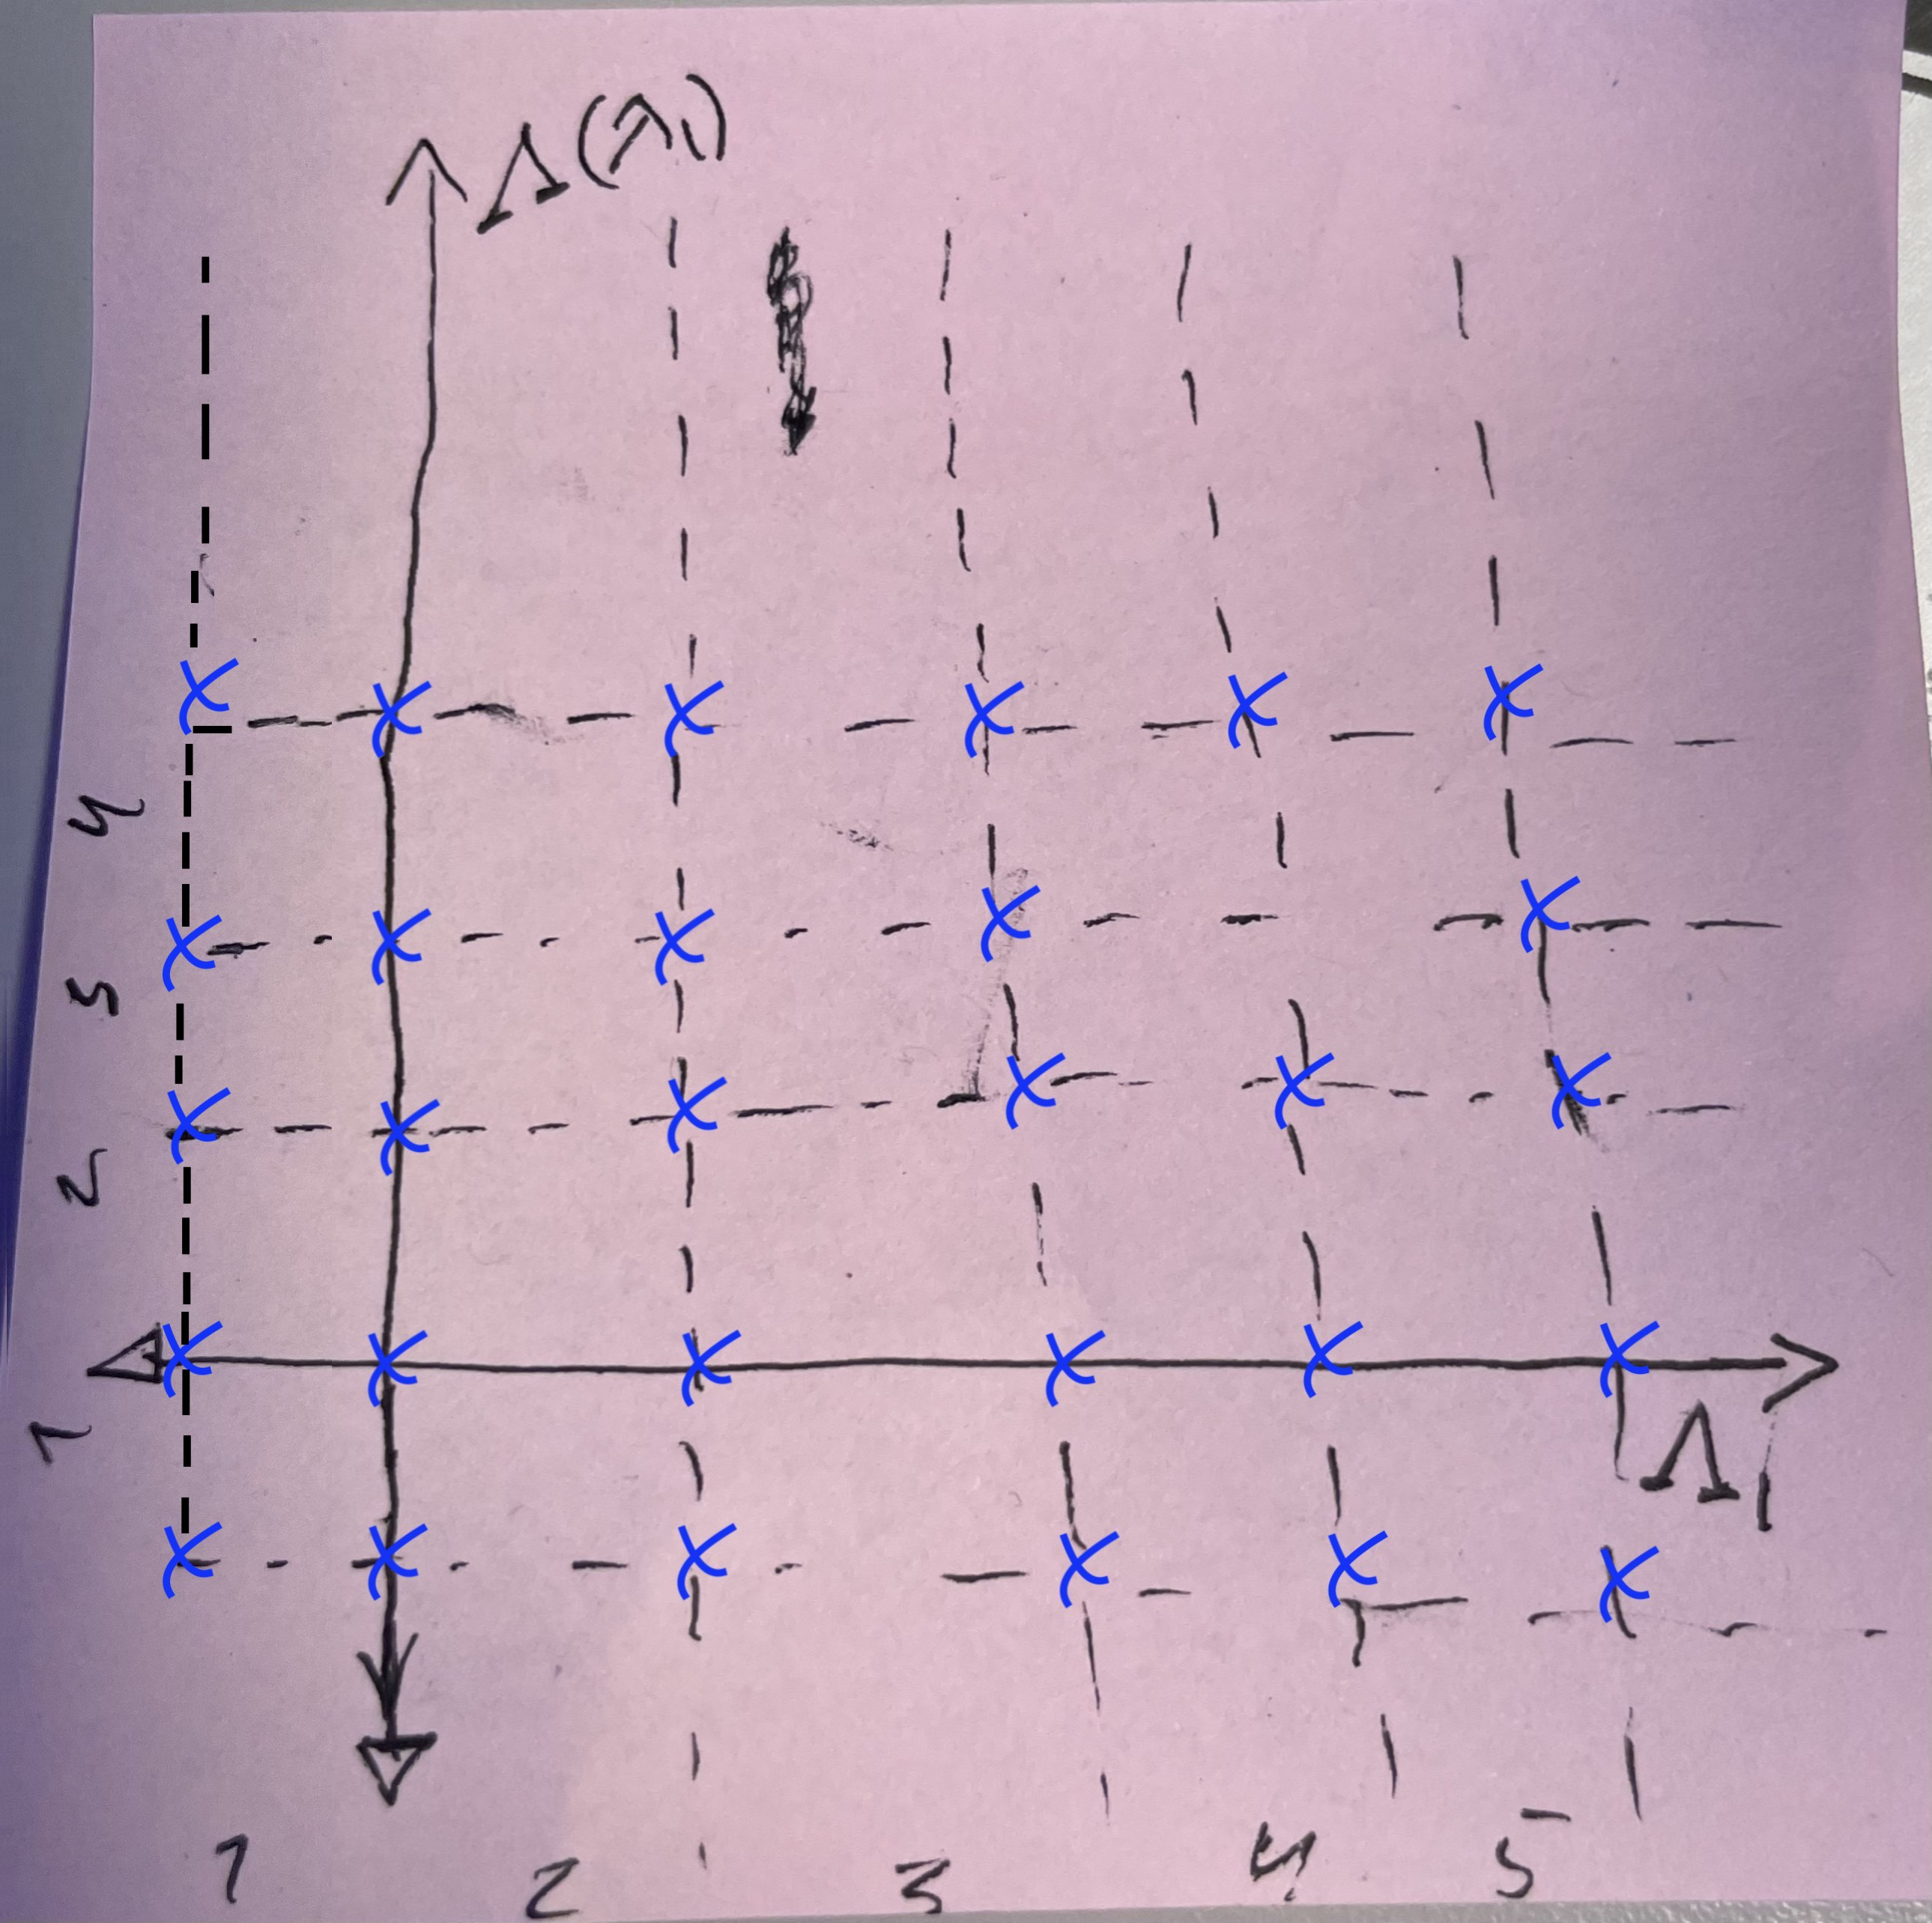
\includegraphics[width=0.9\linewidth]{spec_no_shift.jpg}
        \caption{Lattice spectra}
        \label{fig:lattice_spectra}
    \end{subfigure}\quad
    \begin{subfigure}{.47\textwidth}
        \centering
        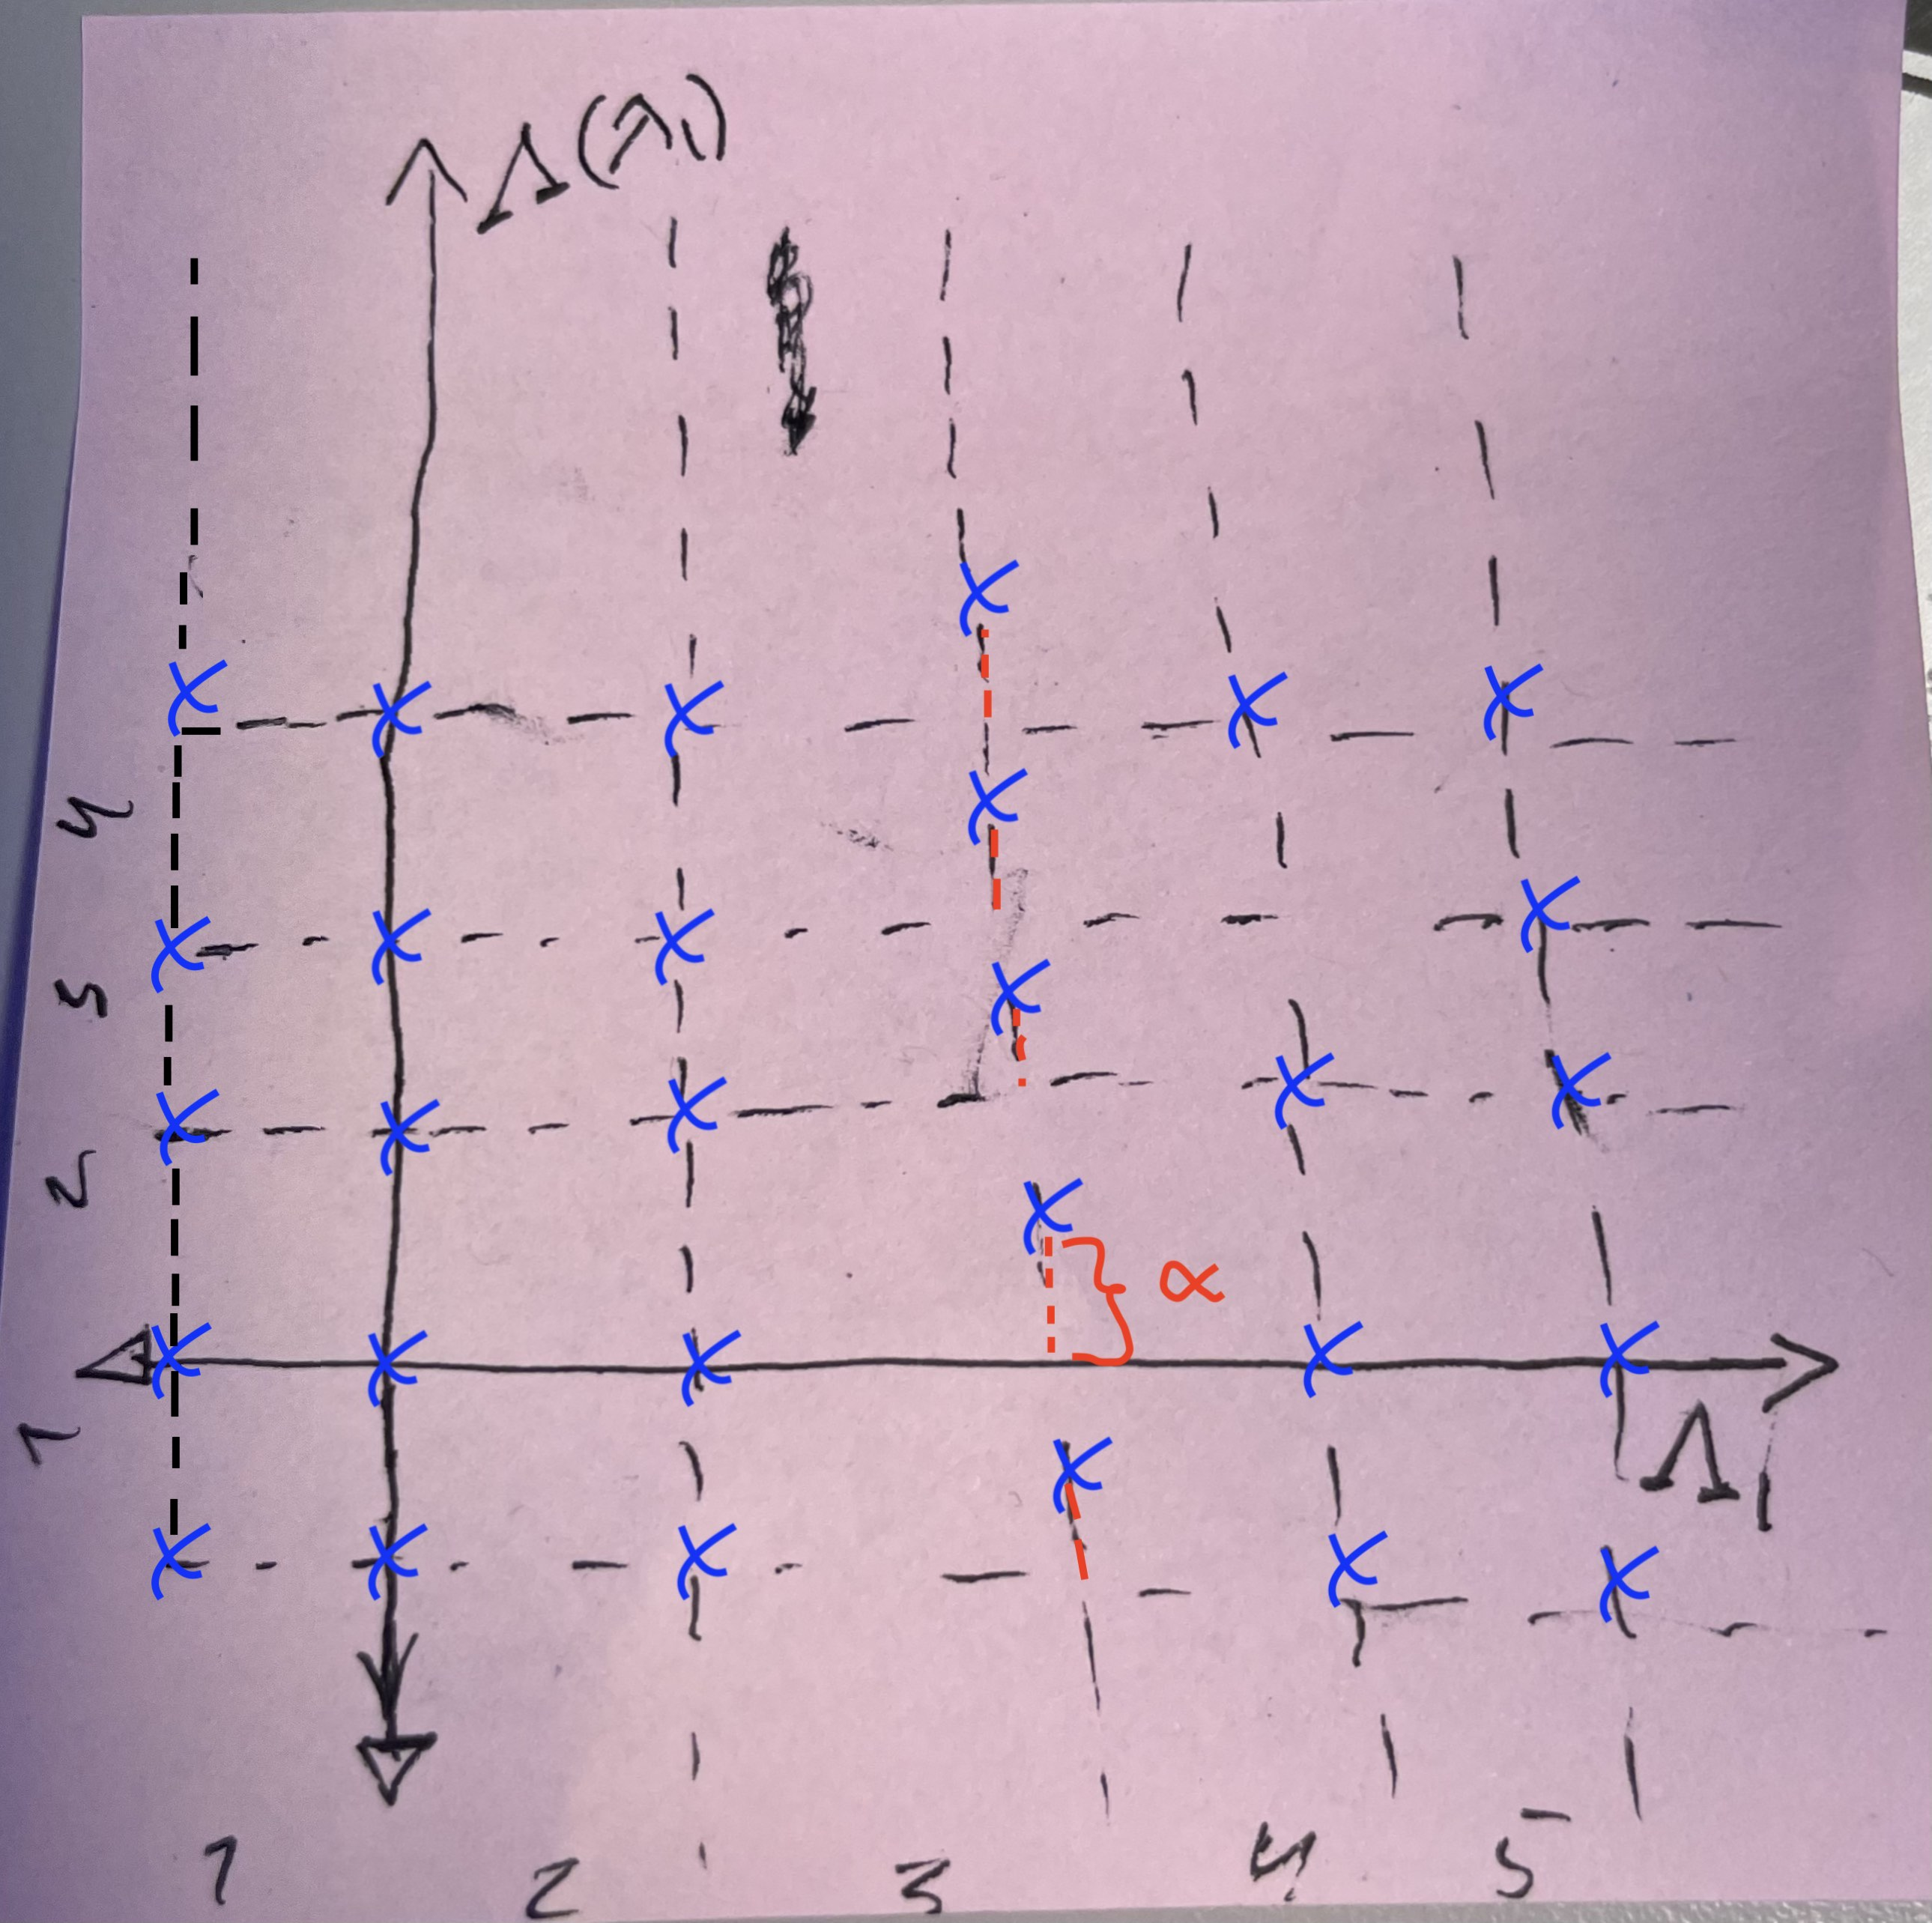
\includegraphics[width=0.9\linewidth]{spec_single_shift.jpg}
        \caption{Single shift vertical}
        \label{fig:single_shift_vertical}
    \end{subfigure}\\
    \begin{subfigure}{.47\textwidth}
        \centering
        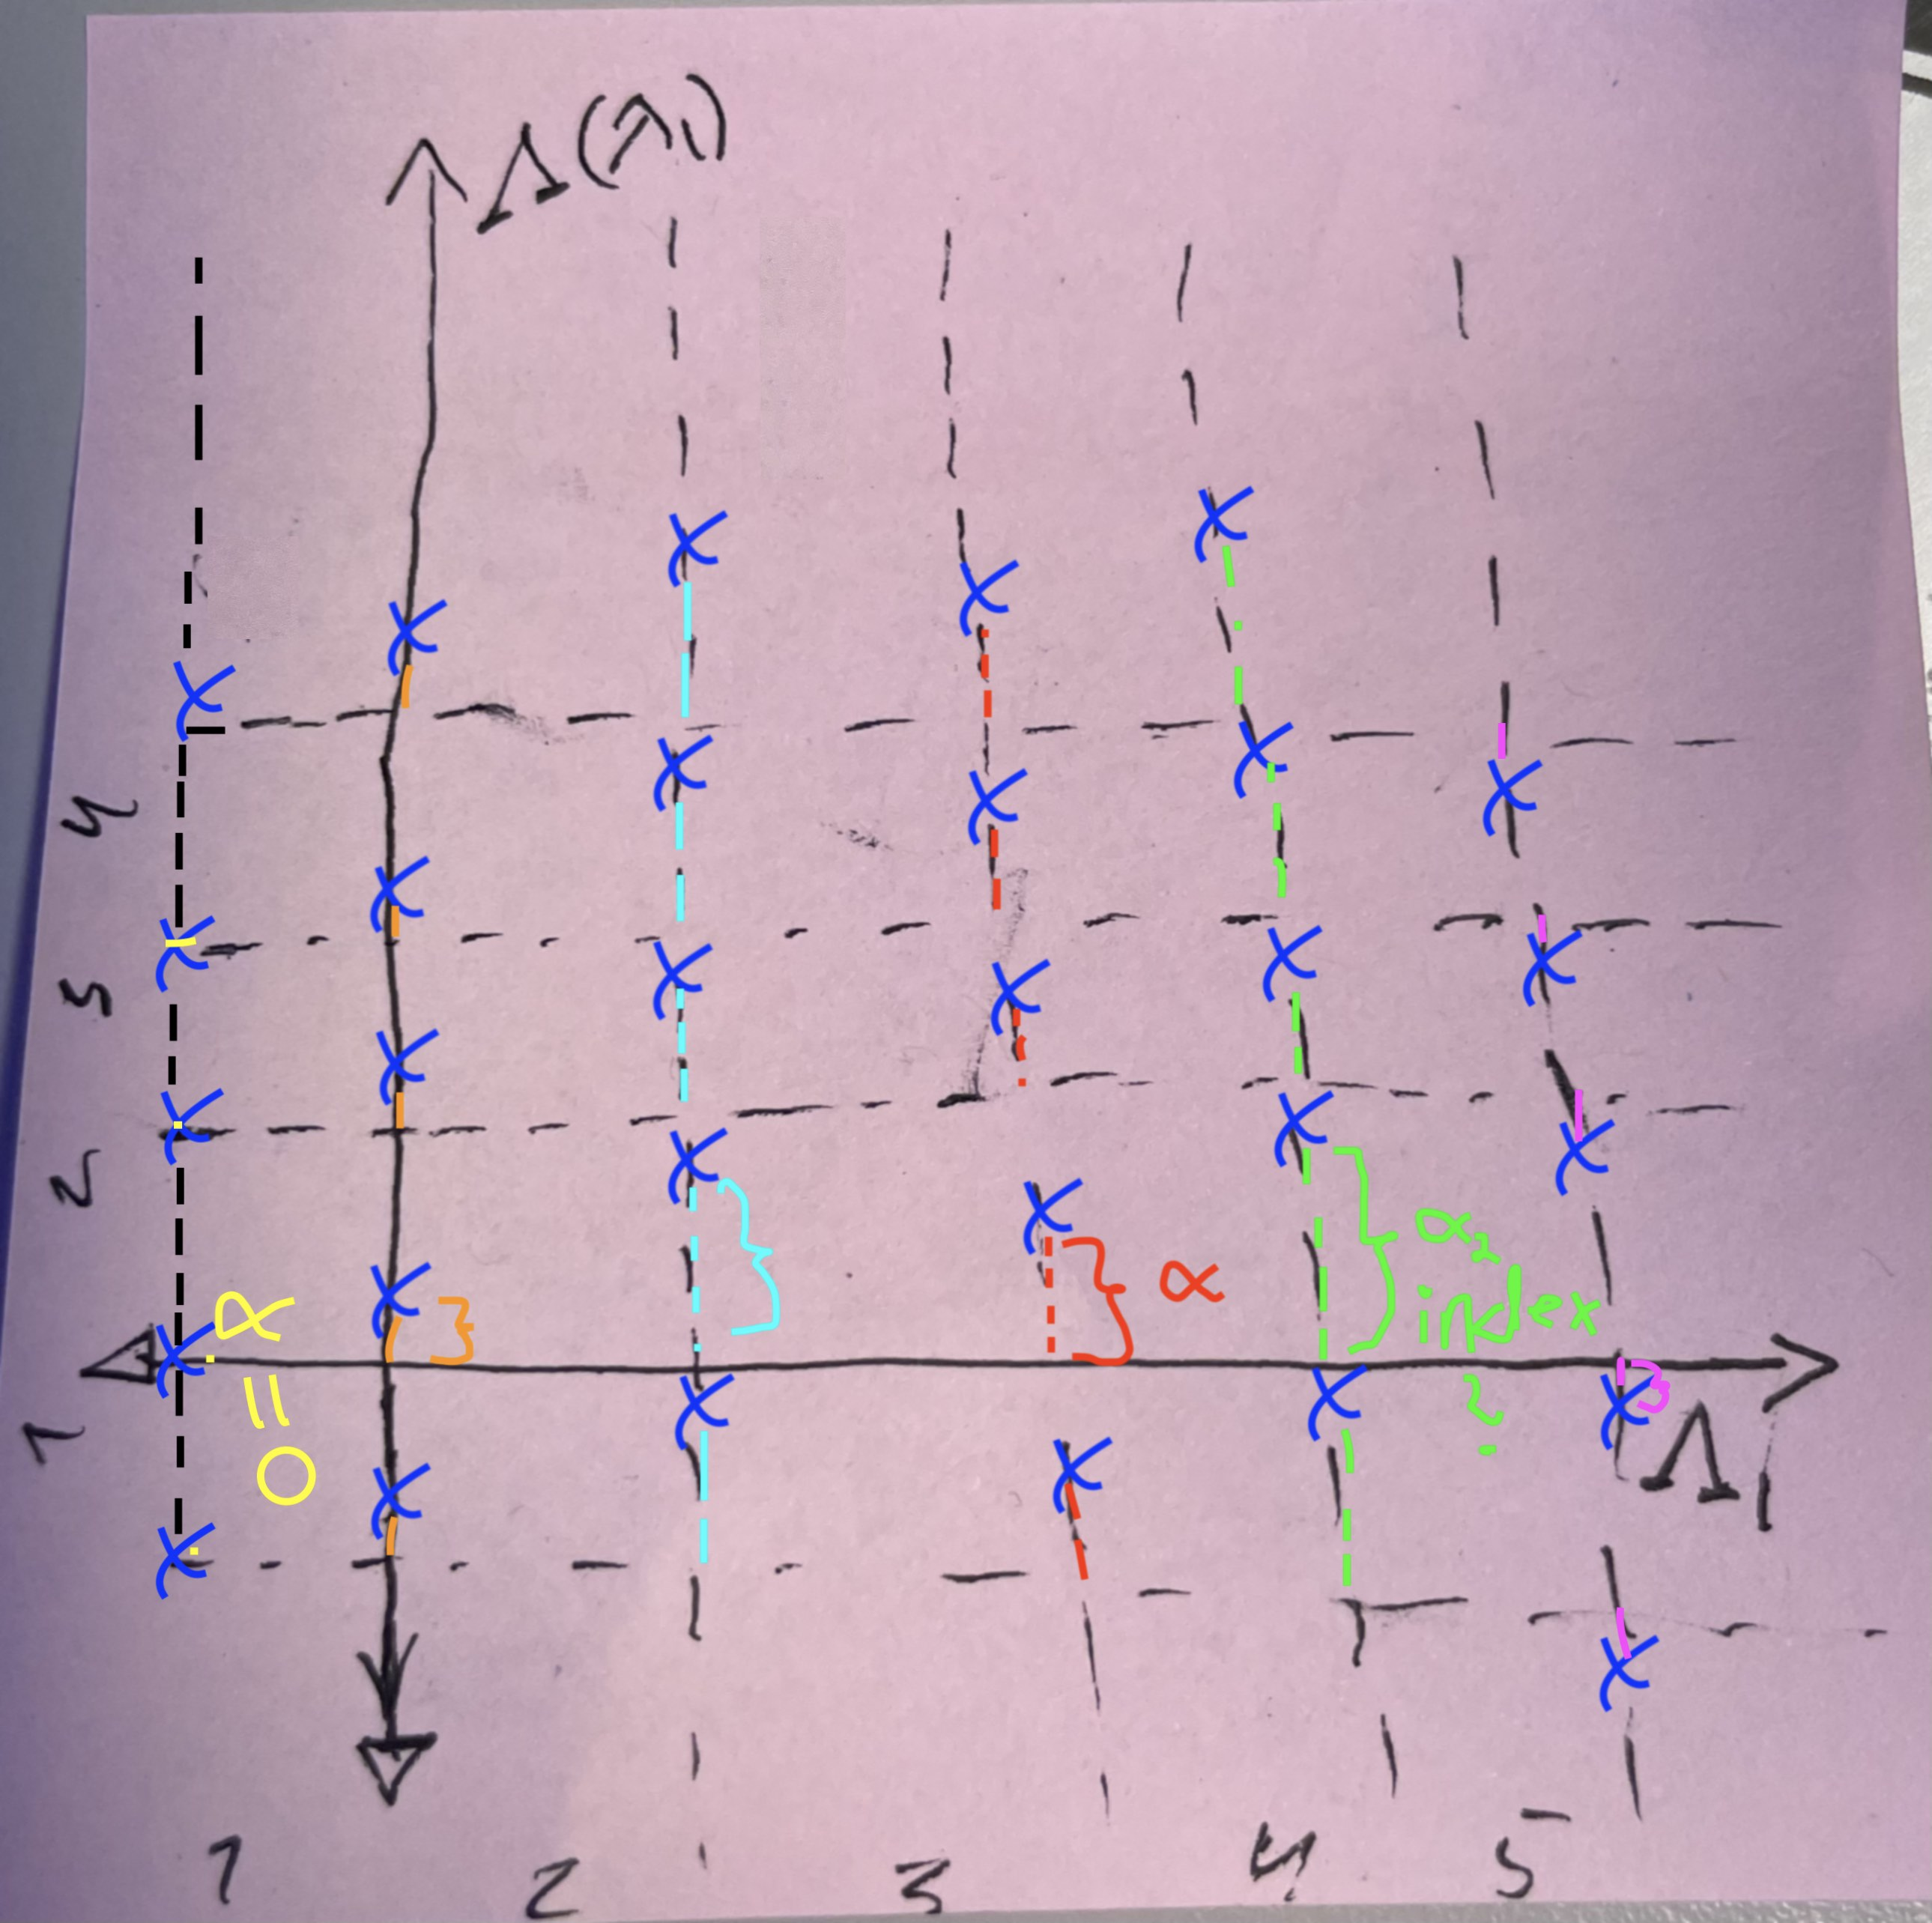
\includegraphics[width=0.9\linewidth]{multiple_shift_left_zero.jpg}
        \caption{Multiple individual shifts vertical}
        \label{fig:multiple_shift_vertical}
    \end{subfigure}\quad
    \begin{subfigure}{.47\textwidth}
        \centering
        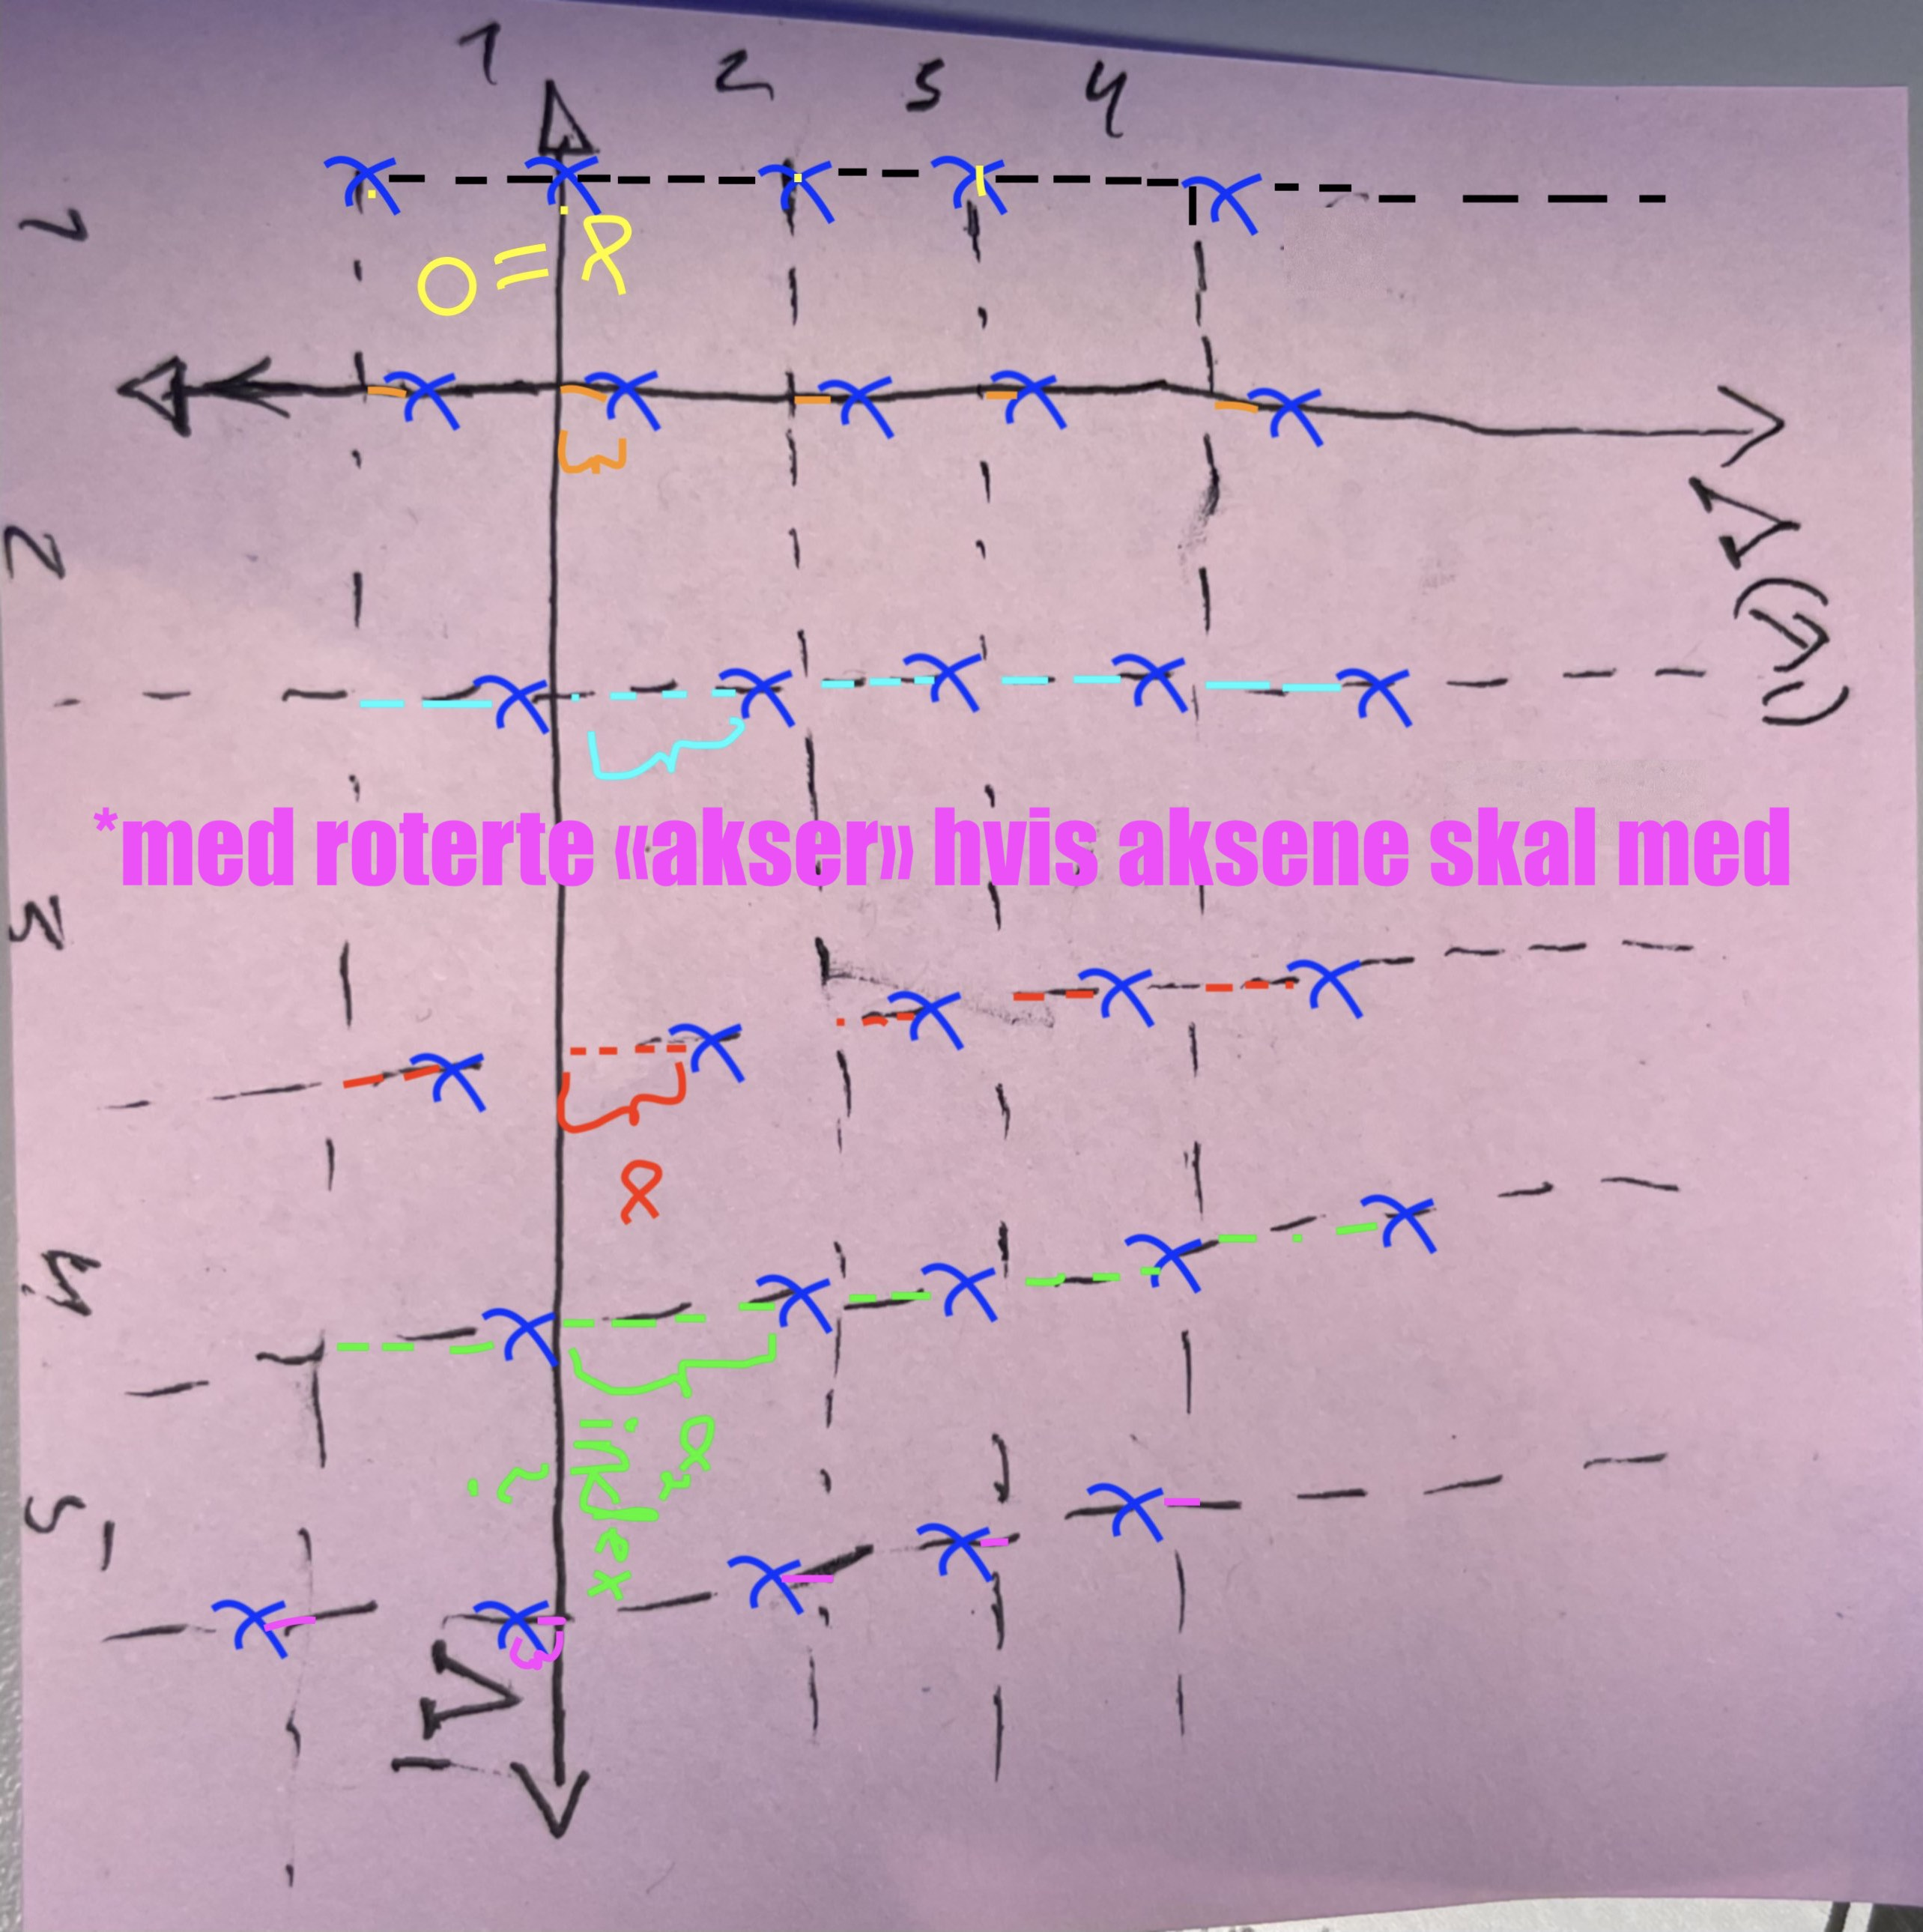
\includegraphics[width=0.9\linewidth]{multiple_shift_left_zero_horizontal.jpg}
        \caption{Multiple individual shifts horizontal}
        \label{fig:multiple_shift_horizontal}
    \end{subfigure}
    \caption{Illustration of the following pair of spectral pairs. In \labelcref{fig:lattice_spectra} we have $\brac{I,\Z}$ and $\brac{I,\lambfunc}$.  In \labelcref{fig:single_shift_vertical} we have $\brac{I,\Z}$ and $\brac{I,\lambfunc}$, where $\lambfunc$ is given by \labelcref{eq:single_shift_vertical}. In \labelcref{fig:multiple_shift_vertical} we have $\brac{I,\Z}$ and $\brac{I,\lambfunc}$, where $\lambfunc$ is given by \labelcref{eq:multiple_shit_func}. In \labelcref{fig:multiple_shift_horizontal} we have $\brac{I,\Z+0.4}$ and $\brac{I,\lambfunc}$, where $\lambfunc$ is given by \labelcref{eq:multiple_shit_func}.}
    \label{fig:spectra_figures}
\end{figure}


As with \cref{prop:class_all_shift}, we can classify all spectra in dimension two as follows. This significant result was proven by Pedersen and Jorgensen in the same paper \cite{jorgensenSpectralPairsCartesian2001}. 

\SigridComment{De nevner $\alpha$ bare som en index, og et "random" tall (ikke R), samt det virker mer som de indekserer med $m,n$ heller en $\alpha$, og det er heller ikke indeks på $\Lambda$ i seg selv for å få frem hva slags skift vi har}
\begin{theorem}\label{thrm:class_all_shift_2d}
    %$\braq{\beta_m \in [0,1) : m \in \Z}$ ANDRE skrivemåten for beta_m
    For a fixed $\alpha \in \R$ and an infinite sequence $\brac{\beta_m}_{m\in \Z}$, $\beta_m \in [0,1)$, the only subsets $\Lambda \subset \R^2$ such that $\Lambda$ is a spectrum for $I^2$ are either one of the two classes:
    \begin{equation}
        \Lambda = \braqMed{
            \begin{pmatrix}
            \alpha + m\\
            \beta_m + n
            \end{pmatrix} : m,n \in  \Z
            }
    \end{equation}
    or
    \begin{equation}
        \Lambda = \braqMed{
            \begin{pmatrix}
            \beta_n + m\\
            \alpha + n
            \end{pmatrix} : m,n \in  \Z
            }
    \end{equation}
    \SigridComment{ekskludert delen om at det også er et tiling set, det er vel hensiktsmessik og splitte disse opp, og komme tilbake til det i neste del, for å så komme med fulle og hele theorem 3.2.} 
\end{theorem}
remark on the half open interval
remark om hvorfor sequencen er essensiell i dette tilfellet for å klassifisere alle skiftene %, samenlignet bare med bare noen random skift


remark om at vi ikke kan ha skift i to retninger, tegne dette

\begin{proof}
    
\end{proof}



\end{document}